\documentclass[UTF8]{ctexart}
\usepackage{graphicx}

\usepackage{ctex}
\CTEXsetup[format={\Large\bfseries}]{section}
\usepackage[top=28mm,bottom=28mm,left=15mm,right=15mm]{geometry}

\usepackage{fancyhdr}
\fancypagestyle{plain}{\pagestyle{fancy}}
\pagestyle{fancy}
\lhead{\kaishu 清华大学药学院药理毒理实验}
\newcommand{\numOfReport}[1]{\rhead{\kaishu 实验报告#1}}

\usepackage{fontspec}
\usepackage{wasysym}
\setCJKmainfont[AutoFakeBold={2}]{STZhongsong}
\setCJKmonofont{STZhongsong}

\usepackage{float}
\usepackage{booktabs}
\usepackage{tabularx}
\usepackage{array}
\usepackage{amsmath}
\usepackage{amsfonts}
\usepackage{amssymb}
\usepackage[figuresleft]{rotating}
\usepackage[para]{threeparttable}
\newcommand\info[2][40mm]{\underline{\makebox[#1][c]{#2}}}
\newcommand{\infoTable}[7]{
    \renewcommand\arraystretch{1.4}
    \begin{table}
        \begin{tabularx}{\textwidth}{
        >{\hsize=0.6\hsize\linewidth=\hsize}X
        >{\hsize=0.6\hsize\linewidth=\hsize}X
        >{\hsize=2.0\hsize\linewidth=\hsize}X
        >{\hsize=0.8\hsize\linewidth=\hsize}X
        }
            天气:\info[14mm]{#1} & 温度:\info[14mm]{#2 $^{\circ}\text{C}$} & 湿度:\info[14mm]{#3 $\%$} & 日期:#4\\
            姓名:\info[14mm]{#5} & 班级:\info[14mm]{#6} & 同组人:\info[70mm]{#7} & 
        \end{tabularx}
    \end{table}
}
\newcommand\columnC{\centering\arraybackslash}
\newcommand\columnL{\raggedright\arraybackslash}
\newcommand\columnR{\raggedleft\arraybackslash}

\usepackage{svg}
\usepackage{pdfpages}

\title{氯丙嗪对小鼠体温的影响}
\author{}
\numOfReport{七}

\begin{document}
\infoTable{小雨}{10}{83}{11/06/2024}{何昱晖}{药3}{荣子健、马逸然、赵方一澜}
\date{}
\maketitle

\section{实验目的及原理}

\subsection{实验目的}

\begin{itemize}
    \item [1] 观察不同环境温度下氯丙嗪对小鼠体温的影响;
    \item [2] 了解氯丙嗪对体温调节的影响及作用特点。
\end{itemize}

\subsection{实验原理}

氯丙嗪是中枢多巴胺受体的阻断剂,具有多种药理活性,包括抗精神病、镇吐、降温等作用。

氯丙嗪能够抑制小丘脑体温调节中枢,使体温调节失灵,不仅能降低发热机体体温,还能降低正常体温,因而机体体温可随外界环境温度变化而改变,出现低或者高的体温状态。在物理降温的配合下,还可使正常体温降至正常水平以下。用较大剂量时,置患者于冷环境中(如冰袋或用冰水浴),可出现「人工冬眠」状态。氯丙嗪用于低温麻醉使可防止休克发生,用于人工冬眠时,与哌替啶、异丙嗪配合冬眠合剂用于创伤性休克、中毒性休克、烧伤、高烧及甲状腺危象的辅助治疗。

\section{实验材料}

\begin{itemize}
    \item 实验动物:健康、雄性小鼠,体重 $18\sim 22\text{g}$;
    \item 药品及试剂:$0.2\%$ 盐酸氯丙嗪溶液、生理盐水、液体石蜡;
    \item 实验器材:电子秤、温度计、冰盒、小鼠固定器、计时器、1mL 注射器。
\end{itemize}

\section{实验方法}

\subsection{室温实验}

每组取 4 只小鼠,称重,标记,随机分为室温给药组(2只)和室温对照组(2只)。先测量给药前每只小鼠的直肠温度。

给药组小鼠腹腔注射 $0.2\%$ 盐酸氯丙嗪(0.1mL/10g),对照组小鼠腹腔注射等体积生理盐水(0.1mL/10g),于注射后第 5、10、15、20、25 和 30min 时测量小鼠体温,并观察记录小鼠的活动情况。

\subsection{低温实验}

每组取 4 只小鼠,称重,标记,随机分为低温给药组(2只)和低温对照组(2只)。先测量给药前每只小鼠在正常室温环境下的直肠温度,然后将小鼠置于固定器中,放置于冰盒中($4\text{C}^\circ$),5min 后取出,测定给药前低温环境下每只小鼠的直肠温度,比较置于冰盒前后小鼠体温的变化。

之后进行给药。给药组小鼠腹腔注射 $0.2\%$ 盐酸氯丙嗪(0.1mL/10g),对照组小鼠腹腔注射等体积生理盐水(0.1mL/10g),注射完成后立即将小鼠置于固定器内,然后再放入冰盒中($4\text{C}^\circ$)。于注射后第 3、5、8、10、15、20min 时测量小鼠体温,并观察记录小鼠的活动情况。

\subsection{注意事项}

\begin{itemize}
    \item [1] 测量小鼠肛温时,体温计探头可先涂抹少量液体石蜡,避免导致出血,避免因操作造成动物挣扎影响体温;
    \item [2] 每次测量肛温时,体温计插入的深度应保持一致,探头整体进入即可;
    \item [3] 低温实验时,注射氯丙嗪后小鼠体温下降很快,部分小鼠 10min 左右体温可降至温度计测量范围以下;
    \item [4] 温度测量间隔较短,建议低温实验和室温实验分开进行。
\end{itemize}

\section{实验结果}

\begin{table}[H]
    \centering
    \begin{threeparttable}[b]
        \caption{室温(20℃)下氯丙嗪对小鼠体温的影响}
        \quad

        \begin{tabularx}{\textwidth}{
            >{\columnC\hsize=1\hsize\linewidth=\hsize}X
            >{\columnC\hsize=1\hsize\linewidth=\hsize}X
            >{\columnC\hsize=1\hsize\linewidth=\hsize}X
        }
        \toprule[1.5pt]
        测量时间 & 氯丙嗪组小鼠平均体温 & 生理盐水组小鼠平均体温 \\
        \midrule
        室温下 & $36.94\pm0.0269$ & $36.97\pm0.0502$ \\
        5min & $34.76\pm0.1037$ & $37.36\pm0.0864$ \\
        10min & $34.21\pm0.0539$ & $37.25\pm0.0896$ \\
        15min & $33.71\pm0.0739$ & $36.87\pm0.0784$ \\
        20min & $33.25\pm0.0553$ & $36.99\pm0.087$ \\
        25min & $32.96\pm0.0623$ & $37.22\pm0.0786$ \\
        30min & $32.62\pm0.041$ & $36.97\pm0.0855$ \\
        \bottomrule[1.5pt]
        \end{tabularx}
    \end{threeparttable}
\end{table}

\begin{table}[H]
    \centering
    \begin{threeparttable}[b]
        \caption{低温(4℃)下氯丙嗪对小鼠体温的影响}
        \quad

        \begin{tabularx}{\textwidth}{
            >{\columnC\hsize=1\hsize\linewidth=\hsize}X
            >{\columnC\hsize=1\hsize\linewidth=\hsize}X
            >{\columnC\hsize=1\hsize\linewidth=\hsize}X
        }
        \toprule[1.5pt]
        测量时间 & 氯丙嗪组小鼠平均体温 & 生理盐水组小鼠平均体温 \\
        \midrule
        室温下 & $36.5\pm0.0682$ & $36.67\pm0.0573$ \\
        给药前 & $34.26\pm0.0768$ & $34.57\pm0.1108$ \\
        5min & $33.67\pm0.0975$ & $33.8\pm0.1187$ \\
        10min & $33.02\pm0.0701$ & $33.42\pm0.1201$ \\
        15min & $32.54\pm0.065$ & $33.54\pm0.0956$ \\
        20min & $32.38\pm0.0483$ & $33.5\pm0.1196$ \\
        25min & $32.06\pm0.0115$ & $33.07\pm0.1013$ \\
        30min & $32.0\pm0.0$ & $32.86\pm0.0867$ \\
        \bottomrule[1.5pt]
        \end{tabularx}
    \end{threeparttable}
\end{table}

\begin{figure}[H]
    \centering
    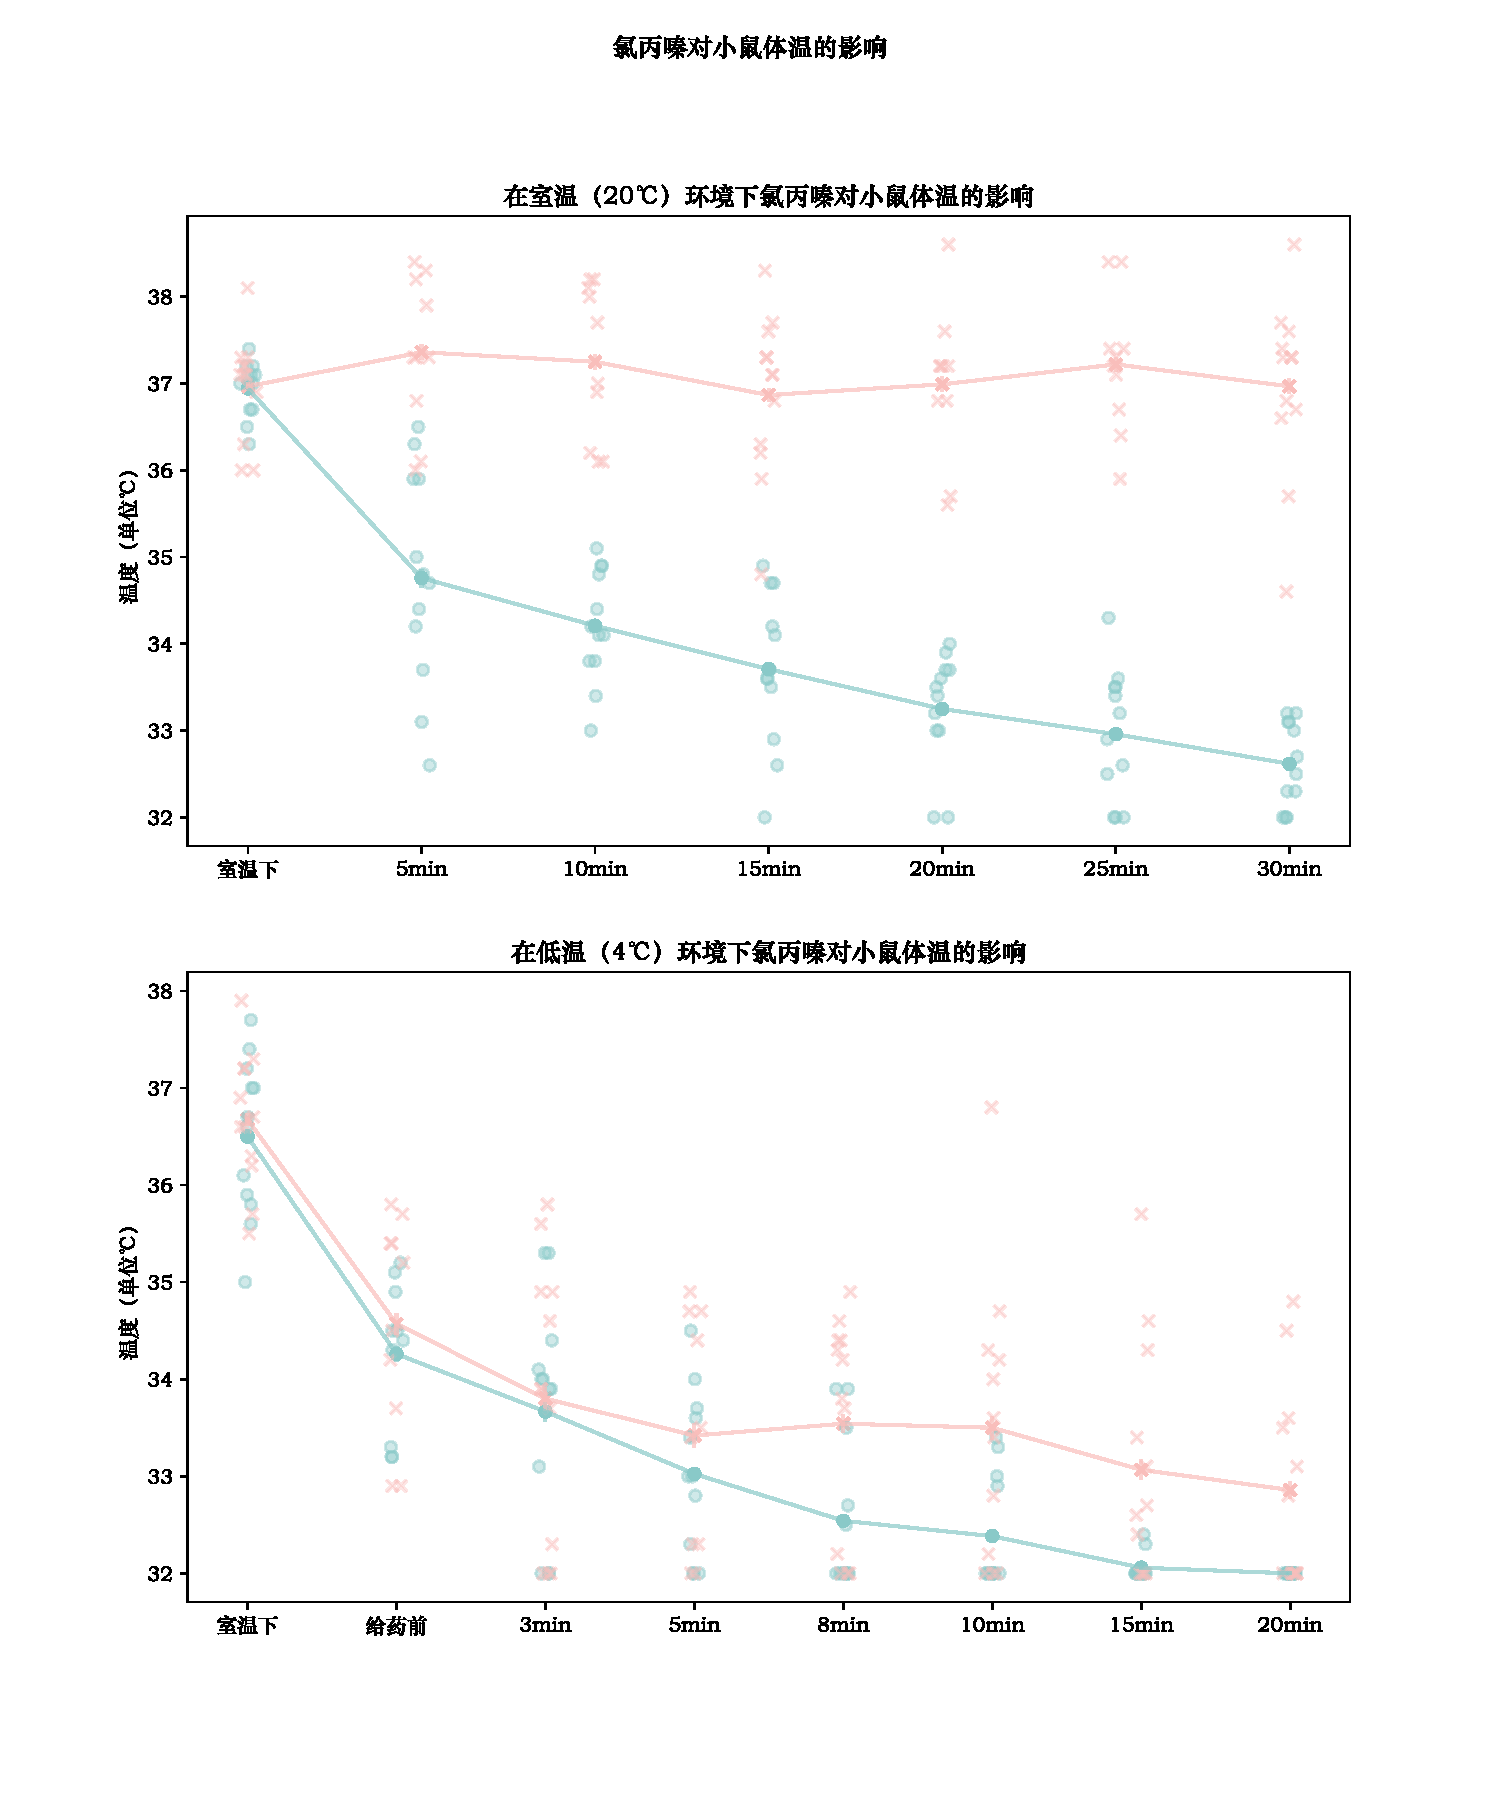
\includegraphics[scale=0.7]{figure-7_svg.pdf}
    \caption{氯丙嗪对小鼠体温的影响}
\end{figure}

\section{课后思考题}

\begin{itemize}
    \item [1] 氯丙嗪影响体温的机制和特点是什么?

        机制是抑制下丘脑体温调节中枢,并且影响其他神经递质的释放和分泌,例如去甲肾上腺素和 5-羟色胺,这些神经递质也参与了体温调节的作用。而氯丙嗪对体温调节具有很强的抵制作用,可以使体温调节功能降低,这同样会消除寒冷反应;

    \item [2] 氯丙嗪与解热镇痛药的解热作用机制有何不同?

        氯丙嗪直接抑制下丘脑体温调节中枢,因此会使正常体温下降;解热镇痛药抑制中枢系统产生的前列腺素而发挥解热作用。

\end{itemize}

\end{document}
